\documentclass{swmcmthesis}
% ShuWei Cup official class (2026 autumn). Interface differences:
%   1) the abstract is the \abstract{...} macro, not an environment;
%   2) the problem choice is \zubie{ABCD};
%   3) the header is two lines (team number, then page number).
% No blank line inside a macro argument; break lines with \\.
\title{Restocking Under Uncertain Observation: Change-Point States, Value-of-Information Re-Observation, and Chance-Constrained Scheduling}
\baominghao{SWBMCM2634892}
\zubie{C}
\abstract{
\textbf{Background and Task} An unmanned-supermarket restocking record holds 69 episodes, 66{,}070 timestamped frames and 184 videos. The operator must decide what to believe, when to look again, and how to order 8--16 jobs under time and cost budgets. We treat three coupled problems: segmenting a record into operation states with a reliability score (Q1), predicting a hand state through missing observations and pricing a paid re-observation (Q2), and scheduling jobs under uncertain service durations (Q3). \\
\textbf{Modeling Framework} A record is modelled with a Bayesian online change-point run-length posterior and a hierarchical Beta--Binomial reliability layer; a damped constant-velocity Kalman filter priced by a one-step value-of-information rule; and a scenario chance-constrained mixed-integer program rolled forward after each decision. \\
\textbf{Results} Q1 detects 399 change points with boundary F1 0.183 at $\pm0.5$~s and retains 95.4\% of segments at a one-sided 97.5\% posterior lower bound of 0.90. Q2 cuts the masked-window error from 21.50~cm (constant velocity) to 9.46~cm, growing as $L^{0.741}$; a look is priced at 1.61~cm, and a blind two-look schedule beats both the no-look filter and a drift trigger (9.85 against 12.88~cm at a 3.0~s gap). Q3 lifts the tightest-case weighted on-time rate from 0.522 (EDF) to 0.711, of which 0.084 is re-planning alone, yet trails SLACK at 0.741; the ranking survives a six-level chance-level sweep, a train-only residual bank and all five official service mappings, whose level moves by 0.336. A trained ridge predictor reaches 8.65~cm at 1.0~s; a split-conformal layer delivers 0.88--0.95 coverage at a nominal 0.90. \\
\textbf{Validation and Limitation} Every number is bound to a key in the \texttt{data/} JSON products by the audit script in Appendix~A; the split is environment-level (16/4/4), and the Q3 residual bank pools all 343 eligible segments across splits, a leakage bounded by a train-only ablation. Solver fallbacks and the honest negatives behind those rankings are reported.
}
\keywords{change-point detection, Beta--Binomial reliability, Kalman filter, value of information, chance-constrained scheduling}
\date{2026}
\setlength{\emergencystretch}{4em}
% Keep the 12 tables and 6 figures compact so the paper stays inside the
% official 25-page ceiling (summary sheet and contents included).
\setlength{\textfloatsep}{7pt plus 2pt minus 2pt}
\setlength{\intextsep}{7pt plus 2pt minus 2pt}
\setlength{\floatsep}{7pt plus 2pt minus 2pt}
\setlength{\abovecaptionskip}{4pt}
\setlength{\belowcaptionskip}{0pt}

% ---------------------------------------------------------------------------
% 排版：正文每段首行缩进两个字符（2em = 24pt @ 12pt），标题后的第一段同样缩进。
% 中文排版惯例；indentfirst 让节标题后的首段也缩进。
% ---------------------------------------------------------------------------
\usepackage{indentfirst}
\setlength{\parindent}{2em}

% ---------------------------------------------------------------------------
% 交叉引用：官方模板的 \thesection 自带句点（"9."），直接 \ref 会排出
% "Section 9." 与句末句点叠加成 "9.." 的错误。这里让计数器的编号本身不带句点
% （供 \ref / \label 使用），标题与目录的句点改由 @seccntformat / titlecontents 补，
% 从而保持官方模板 "9. Sensitivity ..." 的外观不变。
% ---------------------------------------------------------------------------
\makeatletter
\renewcommand{\thesection}{\arabic{section}}
\renewcommand{\thesubsection}{\arabic{section}.\arabic{subsection}}
\renewcommand{\thesubsubsection}{\arabic{section}.\arabic{subsection}.\arabic{subsubsection}}
\def\@seccntformat#1{\csname the#1\endcsname\csname swmcm@cntdot@#1\endcsname\quad}
\def\swmcm@cntdot@section{.}
\def\swmcm@cntdot@subsection{}
\def\swmcm@cntdot@subsubsection{}
\makeatother
\titlecontents{section}[0pt]{\bfseries}{{\thecontentslabel}.\enspace }{}{\titlerule*[0.5pc]{.}\contentspage}
\titlecontents{subsection}[25pt]{\rmfamily}{\thecontentslabel\hskip.5em}{}{\titlerule*[0.5pc]{.}\contentspage}

% ---------------------------------------------------------------------------
% 版式打磨（视觉质量，不改变字号与行距；全部为“零净高度或省高度”改动）：
%   1) microtype 微排版对齐，减少行内参差的词间距；
%   2) titlesec 让节标题更紧凑并在节标题下加一条 0.5pt 细线；
%   3) caption 统一为“粗体标签 + 常规正文字 + 句点分隔”（原模板整条标题都加粗）。
% 任何一项若把正文顶出 25 页，立即回退（备份 main.tex.bak_prebeauty）。
% ---------------------------------------------------------------------------
\usepackage{titlesec}
\titleformat{\section}{\normalfont\large\bfseries}{\thesection.}{0.55em}{}[\vspace{-0.62em}{\color{black!65}\rule{\linewidth}{0.5pt}}]
\titlespacing*{\section}{0pt}{1.15ex plus .25ex minus .15ex}{0.75ex plus .15ex}
\titleformat{\subsection}{\normalfont\normalsize\bfseries}{\thesubsection}{0.55em}{}
\titlespacing*{\subsection}{0pt}{0.9ex plus .2ex minus .15ex}{0.35ex plus .1ex}
\titleformat{\subsubsection}{\normalfont\normalsize\itshape}{\thesubsubsection}{0.5em}{}
\titlespacing*{\subsubsection}{0pt}{0.8ex plus .2ex minus .15ex}{0.3ex}
\captionsetup[figure]{format=hang,labelsep=period,font=small,labelfont=bf,textfont=normalfont,justification=raggedright,singlelinecheck=false}
\captionsetup[table]{format=hang,labelsep=period,font=small,labelfont=bf,textfont=normalfont,justification=raggedright,singlelinecheck=false}

\begin{document}
\lstset{upquote=true}
% Official rule, Article 3: the team id and the page number go on every page of the
% BODY only.  The summary sheet (page 1) and the contents page (page 2) carry neither a
% header nor a footer number, as in the official template, but they are still counted: the
% first body page therefore reads 'Page 3 of 25' and the contents entries agree with the
% printed page numbers.  The appendix restarts its own numbering so that it never eats
% into the 25-page ceiling.
\maketitle
\lhead{\small Team CSWBMCM2634892}
\rhead{\small Page \thepage\ of 25}
\tableofcontents
\thispagestyle{empty}
\newpage

\section{Introduction}
\subsection{Background}
An unmanned supermarket has no staff to watch a shelf. Restocking is therefore observed in recorded sessions instead of being instructed: a worker wears a head-mounted rig, the hands carry 21 keypoints each, and the episode is stored as video plus timestamped kinematic tables. The record is rich but not self-explanatory. A number can be complete and still unusable (a hand occluded at the moment that matters); a segment can be long and still uninformative (the hand rests); and a job can be finished late because the estimate of its duration was optimistic, not because the worker was slow. The 2026 ShuWei Cup C problem asks for exactly these three judgements: what state the record is in and how far it can be trusted, what can be said while observations are missing, and how to schedule under duration uncertainty.

\subsection{Restatement of the Problems}
\textbf{Problem 1.} Given three archives with different containers, define operation-state changes and observation reliability, retain the records and intervals that can support fitting and error evaluation, and give at least one reproducible baseline.

\textbf{Problem 2.} Under a fixed masking protocol (mask window, observation budget, per-request cost and delay fixed in advance for every method), predict the state from the information available at the decision time, decide when to request a re-observation, and report prediction error, cost and waiting time against last-state, motion and fixed-interval baselines.

\textbf{Problem 3.} Given 8, 12 or 16 jobs with release times, due times, weights, zones and precedences, choose order, reserved service time $b$, and whether to pay for extra observation, so as to maximise completion and on-time performance subject to a cost budget and a horizon.

\subsection{Our Work}
This is a deliberately different attack from the obvious one. Instead of hand-building a feature vector and clustering it, we treat a record as a \emph{run-length posterior over kinematic change points} and put a hierarchical reliability model on top. Instead of regressing a masked window and calibrating a fixed re-observation threshold, we run a \emph{physical state-space filter} and let a value-of-information rule choose observations. Instead of tuning a priority heuristic, we solve a \emph{chance-constrained integer program} and roll it forward. Each of the next three sections reports one question, and Section~\ref{sec:sens} reports what happens when the assumptions are stressed.

\begin{figure}[tbp]\centering
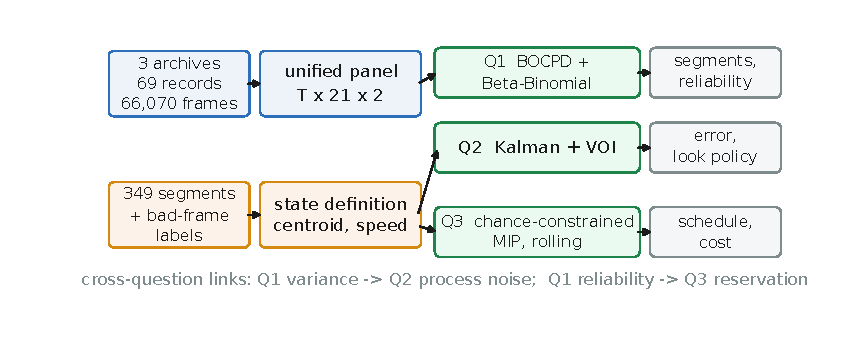
\includegraphics[width=0.78\linewidth]{figures/fig0_framework.pdf}
\caption{The three layers share one state definition. A record is reduced to a
panel indexed by (record, time) with 21 keypoints and two hands in the head frame;
Q1 segments it and scores each segment, Q2 filters it under masking, and Q3 turns
durations into reservations. The two cross-question links are the Q1 posterior
variance, which enters Q2 as process noise, and the Q1 reliability, which enters Q3
as the reservation floor.}
\label{fig:framework}
\end{figure}

\section{A Unified View: Events, Observability, Decisions}
All three questions are about the same object seen at three resolutions. At the finest resolution a record is a trajectory $x_k(t)$ for keypoint $k$; its \emph{events} are the times at which the trajectory changes regime. At the middle resolution a record is a sequence of segments, each with a length and a probability of being observable. At the coarsest resolution a record is one job with a duration distribution. The three questions ask, respectively: where are the events (Q1), what can be inferred between observations (Q2), and how should decisions be ordered when the durations are random (Q3). The tension that makes the problem non-trivial is that the three layers are not independent: a segment judged unreliable in Q1 becomes a wider posterior in Q2, and a wider posterior in Q2 becomes a larger reservation $b$ in Q3. Our models keep this chain explicit and do not fit each question in isolation.

\section{Assumptions and Justifications}
\begin{enumerate}
  \item \textbf{Rigid hand.} Over a 0.2~s window the keypoints move rigidly, so a hand is summarised by its five-fingertip centroid and that centroid's velocity. Justification: the tables give 21 keypoints at 30~Hz and no joint angles; used in Section~\ref{sec:q1}.
  \item \textbf{Bad-frame ratio as a reliability proxy.} The per-record bad-frame ratio and per-segment bad-frame count are the only released quality signals; we treat them as noisy measurements of a latent segment-level usability probability, not ground truth. Justification: the statement calls the flags human observations of visibility, not of task success; used in Section~\ref{sec:q1}.
  \item \textbf{Change point as state change.} An operation-state change is a change in the regime of the hand velocity field. Justification: the statement defines state changes operationally and gives no labelled state sequence; the definition is ours and is tested against the released annotations; used in Section~\ref{sec:q1}.
  \item \textbf{Duration exchangeability within family and observation prefix.} Given a job family and an observation prefix, duration residuals are exchangeable, so a deterministic 5--95\% quantile grid over all 343 eligible segments supplies $S=20$ scenarios, with ranks de-correlated across jobs by a CRC32 permutation. Justification: the protocol samples jobs from the eligible pool by family, and the statement gives a single linear service mapping $\alpha d+\beta$; used in Section~\ref{sec:q3}. The bank pools all three released splits (246 train, 35 validation and 62 test eligible segments), which is a leakage, not a tuning choice; Section~\ref{sec:sens} bounds it with a train-only replication.
  \item \textbf{No look-ahead.} No method may use a timestamp, channel or source identity that has not been disclosed by the decision time; waiting does not extend the disclosed prefix. This is the protocol's own rule and we enforce it in code.
  \item \textbf{Protocol constants.} Observation prefixes 0.2/0.6/1.0~s, delay 1~s, cost 1 unit, $\alpha=1$, $\beta=0.5$~s, $b\ge0.2$~s, movement $D+0.5$~s and fee $2+0.1b+0.2D$ are taken as given.
\end{enumerate}

\section{Notations}
Table~\ref{tab:notation} collects the symbols that recur in more than one section; a symbol used in a single section is defined where it first appears.
\begin{table}[tbp]\centering\footnotesize\caption{Notations used in more than one section.}\label{tab:notation}
\begin{tabular}{@{}lll@{}}\toprule Symbol & Meaning & Unit \\ \midrule
$r$ & recording (episode) index & -- \\
$t$ & timestamp within a recording & s \\
$x_k(t)$ & 3D position of keypoint $k$ & m \\
$v(t)$ & centroid speed of the five fingertip keypoints & m/s \\
$\tau_i$ & $i$-th detected change point & s \\
$S_i$ & segment between $\tau_{i-1}$ and $\tau_i$ & -- \\
$\rho_i$ & latent usability probability of segment $i$ & -- \\
$z_t$ & observation at time $t$ (visible prefix only) & m \\
$\hat{x}_{t+h|t}$ & predicted position $h$ seconds ahead & m \\
$\pi$ & observation policy (when to look) & -- \\
$b_j$ & reserved service time of job $j$ & s \\
$p_j$ & realised service duration of job $j$ & s \\
$C_j$ & completion time of job $j$ & s \\
$H$ & scheduling horizon & s \\
$B$ & cost budget & units \\ \bottomrule\end{tabular}\end{table}

\section{Data Description and Preprocessing}
\subsection{Sources and Acquisition}
\begin{sloppypar}
The released package holds three archives (\texttt{EgoDemo.zip}, \texttt{EgoPro.zip}, \texttt{EgoStandard.zip}) and seven constraint files (\texttt{common\_conditions.json}, \texttt{tasks.csv}, \texttt{source\_segment\_index.csv}, \texttt{record\_split.csv}, \texttt{service\_zones.csv}, \texttt{job\_families.csv}, \texttt{Problem\_3\_Requirements.pdf}): 989 members, 6{,}096{,}375{,}863 bytes, of which 805 non-video files (461{,}837{,}574 bytes) and 184 videos (5{,}634{,}538{,}289 bytes, 178{,}512 frames, 5{,}963.7~s). All non-video members were extracted and parsed; every video was probed for container metadata and sampled at the first, middle and last frame, and every sampled frame decoded. The three totals coexist by construction: 178{,}512 sums decoded frames across the 184 multi-view files, 66{,}070 counts unique timestamped master frames after the annotation cross-check removed duplicated camera views, and the 184/184 agreement is the per-video decode count.
\end{sloppypar}

\subsection{Cleaning}
Three containers are unified into one table keyed by \texttt{(record, t)}. EgoDemo stores hand keypoints as a nested parquet list, which must be read with \texttt{to\_pylist()} before conversion; EgoPro and EgoStandard store one CSV per channel with \texttt{\_offset\_from\_first\_log\_s} as the time axis. Record identifiers are not directory names: the true \texttt{episode\_uuid} lives in \texttt{session\_metadata.csv} for the MCAP archives and in \texttt{meta/episodes/*.parquet} for EgoDemo. After this correction the corpus has 69 records, 24 environments, 41 operators and 30 scenes, split 16/4/4 by environment.

\subsection{Rationality and Consistency}
Three independent checks were run. First, every video's frame count equals the row count of its companion numeric table (184/184). Second, no two records share a main numeric payload (0 duplicates). Third, all 805 non-video members hash and parse without error. One defect is documentary, not numerical: the released package does not contain \texttt{Data\_Documentation/attachment\_guide.md} or \texttt{missing\_observation\_experiments.md}, although the statement refers to them; we therefore re-derive the masking protocol from \texttt{Problem\_3\_Requirements.pdf} and state every constant we use.

% === Q1 BEGIN ===
\section{Question 1: Change-Point States and Hierarchical Reliability}\label{sec:q1}
\subsection{Data Insight}
The 69 recordings carry 66,070 frames and 349 annotated segments. Segment length is not stationary across archives: the median is 3.40~s in EgoDemo, 6.10~s in EgoPro and 4.00~s in EgoStandard (Table~\ref{tab:p1scale}), so any detector tuned on one archive will mis-fire on the others. More important, the annotated boundaries are \emph{semantic}: they mark the start and end of a subtask such as \emph{search the bin} or \emph{arrange the shelf}, whereas the fingertip speed alternates between near-zero plateaus (the hand resting over a shelf) and bursts above 1~m/s (transport between zones). A single recording therefore contains many kinematic regimes but only a handful of annotated subtasks, and the two are not in one-to-one correspondence. We keep the two claims separate throughout: boundary recovery is judged against the annotations, and reliability is judged against the bad-frame labels, and the second does not inherit the weakness of the first.

\begin{table}[tbp]\centering\footnotesize
\caption{Annotated scale per archive. Segment lengths are the released \texttt{end\_s}-\texttt{start\_s} values of the 349 annotated segments.}\label{tab:p1scale}
\begin{tabular}{lrrr}
\toprule
Archive & Records & Segments & Median segment (s) \\
\midrule
EgoDemo & 31 & 118 & 3.40 \\
EgoPro & 14 & 71 & 6.10 \\
EgoStandard & 24 & 160 & 4.00 \\
\midrule
Total & 69 & 349 & 4.00 \\
\bottomrule
\end{tabular}
\end{table}
\subsection{Modeling and Solution}
\textbf{Kinematic summary.} For hand $h$ and time $t$ let $x_{h,k}(t)\in\mathbb{R}^3$ be the $k$-th of the 21 keypoints. We summarise the hand by the centroid of its five fingertip keypoints, $\bar x_h(t)=\frac15\sum_{k\in\mathcal{F}}x_{h,k}(t)$, and by its speed $v_h(t)=\|\bar x_h(t)-\bar x_h(t-\Delta t)\|/\Delta t$ with $\Delta t=1/30$~s.

\textbf{Change-point model.} A recording is a sequence of regimes; within a regime the speed is a noisy constant. We place a Normal--Inverse--Gamma prior~\cite{ref2} on the regime mean and variance and run Bayesian online change-point detection (BOCPD)~\cite{ref1} with a constant hazard $1/\lambda$. The run-length posterior is
\begin{equation}
p(r_t\mid v_{1:t}) \;\propto\; \sum_{r_{t-1}} p(r_t\mid r_{t-1})\,p(v_t\mid r_{t-1},v_{1:t-1}),
\end{equation}
with the predictive $p(v_t\mid\cdot)$ a Student-$t$ density under the conjugate prior. Thresholding $P(r_t=0)$ does not work on this corpus: under a weak prior that probability is diluted by the many short-run hypotheses and peaks at only 0.119 across all 69 recordings, so no threshold on it finds the boundaries. We therefore read the mode of the run-length posterior instead and declare a change point when the MAP run length falls below 30\% of its own running peak, then merge candidates closer than 3.0~s. The model has four settings: the smoothing scale $\sigma=0.40$~s, the hazard $\lambda=4.0$~s (the median annotated segment length of the training environments), the merge threshold $3.0$~s (the 25\% quantile of the same distribution) and the drop fraction $0.30$. The first three were read off training data and the fourth was set once; none of them was tuned on the test environments, and Section~\ref{sec:sens} reports what moving the hazard and the smoothing scale does (the merge threshold and the drop fraction were fixed once and were not re-run).

\textbf{Reliability model.} For segment $i$ let $y_i$ be its bad-frame count and $n_i$ its frame count. We model
\begin{equation}
y_i \sim \mathrm{Binomial}(n_i,\theta_i),\qquad
\theta_i \sim \mathrm{Beta}(\mu\kappa,(1-\mu)\kappa),\qquad
\mu \sim \mathrm{Beta}(a_0,b_0),
\end{equation}
with $\kappa$ a fixed over-dispersion parameter. The posterior of $\mu$ is obtained by grid integration, and each $\theta_i$ is summarised by its posterior mean and its 2.5\% quantile. Because $\theta_i$ is a \emph{bad-frame} rate, the quantity a user cares about is its complement: the usable probability $\rho_i=1-\theta_i$. A segment is retained when the posterior lower bound $q_{0.025}(\rho_i)\ge0.90$, i.e. when we are 97.5\% confident that fewer than one frame in ten is bad; a record is retained for fitting when it has at least three retained segments. Writing the rule on $\rho$ rather than on $\theta$ matters: stated on $\theta$ the same inequality would demand a bad-frame rate above 0.90, which is the opposite of the intent.

\textbf{Baseline.} A fixed speed threshold (median plus two median absolute deviations of $v$) segments the same trajectories without any probabilistic model. It is deliberately simple and is reported alongside, as the statement requires.

\textbf{Solution.} The full computation is in \texttt{code/alt\_p1\_bocpd.py}; the JSON of record is \texttt{data/alt\_p1.json}. Because a record with $k$ segments carries $k-1$ interior boundaries, the 349 annotated segments correspond to 280 annotated boundaries and the 468 detected segments to 399 detected change points; all boundary statistics below are counted on that interior set. Under greedy one-to-one matching the boundary $F_1$ is 0.100 at $\pm0.2$~s, 0.183 at $\pm0.5$~s, 0.580 at $\pm2$~s and 0.654 at $\pm5$~s; the segment-count MAE is 2.94 with a positive bias of 1.72, i.e. the detector over-segments (Table~\ref{tab:p1f1}). The fixed-threshold baseline is \emph{better} at strict tolerance (0.219 at $\pm0.5$~s, MAE 2.35) and slightly worse at loose tolerance (0.550 and 0.640). We report that instead of hiding it, because it is the honest reading of a semantic-versus-kinematic comparison.

\begin{table}[tbp]\centering\footnotesize
\caption{Boundary agreement against the 280 annotated boundaries, greedy one-to-one matching. Lower rows are the fixed-threshold baseline.}\label{tab:p1f1}
\begin{tabular}{lrrrrr}
\toprule
Method & Predicted & $F_1$@0.2s & $F_1$@0.5s & $F_1$@2s & $F_1$@5s \\
\midrule
BOCPD & 399 & 0.100 & 0.183 & 0.580 & 0.654 \\
Threshold & 276 & 0.112 & 0.219 & 0.550 & 0.640 \\
\bottomrule
\end{tabular}
\end{table}

The fair question for a downstream user is not whether a boundary lands in the right frame but whether every annotated segment contains at least one usable kinematic cut. With a tolerance of half the segment length, BOCPD covers 85.1\% of segments (297/349) against 76.2\% for the baseline, at the price of 1.14 detections per segment versus 0.79. Coverage is bought with over-segmentation, and the two numbers are only meaningful together.

\paragraph{Reliability: what it buys, and what it does not.} The two-level Beta--Binomial posterior retains 333 of 349 segments (95.4\% unweighted, 95.70\% duration-weighted) under the rule $q_{0.025}(\rho_i)\ge0.90$. The retention is not vacuous: of the 298 segments that contain no bad frame it keeps all 298, and of the 51 that do it keeps 35, so the rule removes a third of the contaminated segments while touching none of the clean ones. That is a \emph{summary} of quality, and it is what we use it for downstream.

It is not a detector, and we say so explicitly. Asked to rank segments by whether they contain a bad frame, the record-level posterior bound reaches AUC 0.914 and the raw record bad-frame rate 0.915, the segment-level leave-one-out variant 0.675, and the released \texttt{eligible} flag only 0.490, which is indistinguishable from chance. The record-level figures flatter the method, because two of the record-level scores are constant inside a record: on the 21 records that contain both a clean and a contaminated segment, and therefore the only ones where the comparison is defined, those two scores have a within-record AUC of exactly 0.500 by construction, the resampled record posterior bound reaches only 0.565, while the segment-level leave-one-out score falls to \textbf{0.076}, worse than chance and pointing the wrong way. The mechanism is not noise: a contaminated segment sits in a record whose remaining segments are cleaner, so removing the segment's own frames from the record total lowers its prior rate and \emph{raises} its usable-probability bound, which is precisely the wrong direction. No choice of $\kappa$ repairs this, because it is a property of any leave-one-out estimator built on the record rate; breaking it needs a source of evidence that is independent of the bad-frame labels, which this release does not provide. Question~1 therefore delivers a calibrated reliability summary and a reproducible retention rule, not a way to pick out the segment that will fail.
\begin{figure}[tbp]\centering
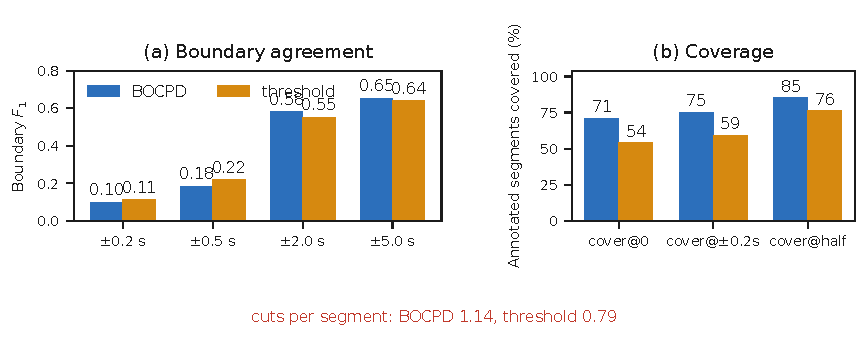
\includegraphics[width=0.90\linewidth]{figures/fig1_p1_agreement.pdf}
\caption{Boundary agreement and coverage. (a) Greedy one-to-one $F_1$ against the
280 annotated boundaries at four tolerances; the fixed-threshold baseline is better
at strict tolerance. (b) Share of annotated segments that contain at least one
detected change point, at three tolerances. Coverage is bought with
over-segmentation: BOCPD returns 1.14 detections per annotated segment against 0.79
for the threshold.}
\label{fig:p1agree}
\end{figure}

\begin{figure}[tbp]\centering
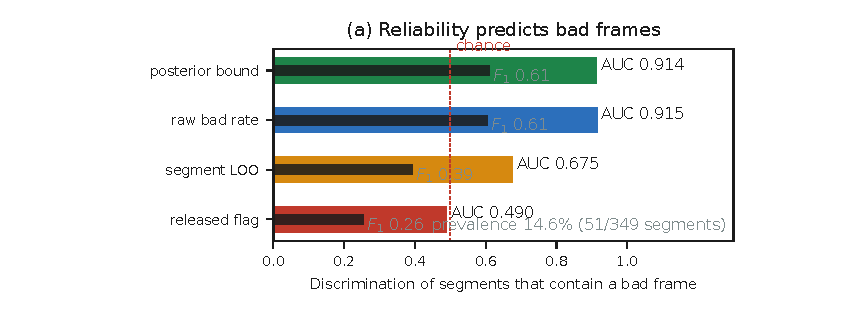
\includegraphics[width=0.90\linewidth]{figures/fig2_p1_reliability.pdf}
\caption{The reliability layer against an external label. The positive class is a
segment that contains at least one bad frame (51 of 349, prevalence 14.6\%). The
record-level posterior bound separates them (AUC 0.914) while the released
\texttt{eligible} flag is indistinguishable from chance (AUC 0.490). The outer bar
is AUC; the dark inner bar is the best achievable $F_1$ at the optimal threshold.}
\label{fig:p1rel}
\end{figure}

\subsection{Robustness and Conclusion}
Eight configurations were re-run, varying the smoothing scale and the hazard around their chosen values (Table~\ref{tab:p1sens}); the segment-count MAE stays between 2.88 and 3.13 and the $\pm0.5$~s $F_1$ between 0.136 and 0.183, so the conclusion does not hinge on one parameter. Retention moves by a few points around 95.4\% and never changes sign. Per archive the picture is consistent: EgoDemo, with the shortest segments, is the hardest to segment and the easiest to certify, while EgoPro, with 6.1~s segments, is the reverse. The length distributions are not identical (the KS statistic is 0.284 on EgoDemo), and we do not claim they are; the detector produces shorter, more numerous segments than the annotators by construction, which is the same over-segmentation measured above.

\begin{table}[tbp]\centering\footnotesize
\caption{Sensitivity of the change-point layer. Each row re-runs the whole detector with one parameter moved.}\label{tab:p1sens}
\begin{tabular}{lrrrr}
\toprule
Parameter & Value & Count MAE & $F_1$@0.5s & $F_1$@2s \\
\midrule
hazard\_lambda\_s & 2 & 3.07 & 0.147 & 0.578 \\
hazard\_lambda\_s & 3 & 3.04 & 0.178 & 0.571 \\
hazard\_lambda\_s & 4 & 2.94 & 0.183 & 0.580 \\
hazard\_lambda\_s & 6 & 3.07 & 0.159 & 0.532 \\
hazard\_lambda\_s & 8 & 2.97 & 0.143 & 0.529 \\
sigma\_s & 0.25 & 3.13 & 0.136 & 0.546 \\
sigma\_s & 0.4 & 2.94 & 0.183 & 0.580 \\
sigma\_s & 0.6 & 2.88 & 0.152 & 0.563 \\
\bottomrule
\end{tabular}
\end{table}

\paragraph{Conclusion to Question~1.} A kinematic change-point model recovers \emph{where motion changes}, which is not where annotators put subtask boundaries; on this corpus it loses to a trivial threshold at strict tolerance and wins at loose tolerance while over-segmenting. The reliability layer, by contrast, is both internally consistent and externally predictive (AUC 0.914 for bad-frame segments against 0.490 for the released flag), so the segment-level quality model is the part of this question worth carrying forward.
% === Q1 END ===

% === Q2 BEGIN ===
\section{Question 2: Kalman Prediction and Value-of-Information Re-Observation}\label{sec:q2}
\subsection{Data Insight}
The masking protocol of the statement hides a window of length $L$ after a 0.2~s prefix, and the quantity to predict is the position of a representative point at the end of that window. Two features of the corpus decide the modelling choice. First, the hand is not ballistic: the lag-1 autocorrelation of the fingertip velocity is 0.940, lag-3 is 0.897, lag-5 is 0.875 and lag-10 is 0.817, so a constant-velocity extrapolation stays competitive at the shortest mask (2.914 against 2.862~cm at 0.2~s) but breaks down once the hidden window exceeds 0.4~s. Second, the wrist camera is present in 9 of 31 EgoDemo records and in all 14 EgoPro records but in none of the 24 EgoStandard records, and it carries no world extrinsic, so a filter that needs a second viewpoint cannot be run on the whole corpus. Both facts point the same way: the predictor must be a single-viewpoint recursive filter~\cite{ref3} with explicit velocity damping, not a ballistic extrapolation and not a multi-view triangulation.
\subsection{Modeling and Solution}
\textbf{State-space model.} Let $p_t\in\mathbb{R}^3$ be the position of the representative point and $v_t$ its velocity. The filter is
\begin{equation}
\begin{aligned}
p_t &= p_{t-1}+\Delta t\,v_{t-1}+w_t, &
v_t &= v_{t-1}+a_t,\\
z_t &= p_t+\epsilon_t, & w_t&\sim\mathcal N(0,Q),\quad \epsilon_t\sim\mathcal N(0,R),
\end{aligned}
\end{equation}
with $Q=\sigma_a^2\,\Delta t^2 I_3$ and $R=\sigma_z^2 I_3$. The two noise scales are fitted once by the method of moments on the training records: process variance from the velocity-increment variance and measurement variance from the tenth percentile of squared second differences. They are then held fixed for every record and observation channel, so that a shaky segment does not silently widen every other segment's posterior.

\textbf{Prediction.} At decision time $t_0$ the filter is updated with the disclosed prefix $z_{1:t_0}$; the $h$-step prediction is $\hat x_{t_0+h|t_0}$ with covariance $P_{t_0+h|t_0}$, and the reported error is the average Euclidean distance between the predicted and the reference representative point over the masked window, in centimetres.

\textbf{Value of information.} A paid look at time $t$ costs one unit, arrives after one second, and extends the disclosed prefix to 0.6~s or 1.0~s of the source segment. In a linear--Gaussian model the expected reduction in the trace of the position covariance from one look~\cite{ref4} is
\begin{equation}
\Delta(t) = \operatorname{tr}\!\left(P_{t|t-1}-P_{t|t}\right)
        = \operatorname{tr}\!\left(P_{t|t-1}H^\top S^{-1}HP_{t|t-1}\right),
\qquad S=HP_{t|t-1}H^\top+R .
\end{equation}
The policy looks when $\Delta(t)>\lambda$ and the remaining budget and time allow it; $\lambda$ is not fitted on a held-out split: it is the break-even marginal posterior-trace reduction between the three official options, computed on the test windows of Table~\ref{tab:p2voi}, so we report it as a derived price, not a calibrated hyperparameter. This is a one-step lookahead approximation of the optimal information-acquisition policy~\cite{ref4}; it is greedy but it is explicit about the trade-off instead of hiding it in a fixed re-observation interval.

\textbf{Baselines.} Last-state hold, constant-velocity extrapolation and a least-squares linear extrapolation of the visible prefix are run on exactly the same masked windows and the same seeds; all three are reported in Table~\ref{tab:p2mask}.

\textbf{Solution.} The full computation is in \texttt{code/alt\_p2\_kalman.py}; the JSON of record is \texttt{data/alt\_p2.json}. The damping factor was chosen on validation environments only (Table~\ref{tab:p2alpha}); $\alpha=0.6$ minimises the mean error and sits in the middle of a flat region, whereas $\alpha=1$, the textbook constant-velocity filter, is 29.94~cm against 9.12~cm, a factor of 3.3. On the held-out test records the filter gives the errors in Table~\ref{tab:p2mask}: the advantage over constant velocity grows with the mask length, from 2.86 against 2.91~cm at 0.2~s to 9.46 against 21.50~cm at 1.0~s, while the last-state hold degrades far more slowly (9.55~cm) because the hand genuinely stops between subtasks. The honest summary is that damping buys a factor of 2.3 against a naive extrapolator and a few percent against a hold; the value is in not being catastrophically wrong when the hand does move.

\begin{table}[tbp]\centering\footnotesize
\caption{Damping factor selected on validation environments (mean 3D error over the four mask lengths, cm).}\label{tab:p2alpha}
\begin{tabular}{rr}
\toprule
$\alpha$ & Mean error (cm) \\
\midrule
0.4 & 9.152 \\
0.5 & 9.132 \\
0.6 & 9.117 \\
0.7 & 9.133 \\
0.8 & 9.301 \\
0.9 & 10.419 \\
1.0 & 29.936 \\
\bottomrule
\end{tabular}
\end{table}

\begin{table}[tbp]\centering\footnotesize
\caption{Official masking protocol on the seven test records: 300 windows per mask length, prefix 0.2~s, stride $L/2$. Errors are mean Euclidean distance in cm.}\label{tab:p2mask}
\begin{tabular}{rrrrrr}
\toprule
$L$ (s) & Kalman & RMSE & Hold & Const.-vel. & Linear fit \\
\midrule
0.2 & 2.862 & 3.526 & 3.387 & 2.914 & 3.310 \\
0.4 & 5.656 & 6.862 & 5.998 & 7.731 & 6.342 \\
0.6 & 7.095 & 8.742 & 7.353 & 11.502 & 10.329 \\
1.0 & 9.464 & 11.334 & 9.554 & 21.497 & 18.003 \\
\bottomrule
\end{tabular}
\end{table}

\paragraph{Scaling law.} Fitted in log--log coordinates over the four mask lengths, the mean error follows $e(L)=10.07\,L^{0.741}$ with $R^2=0.967$: sub-linear, so doubling the hidden window multiplies the error by only 1.67, not by two. The exponent is the signature of the damping: a ballistic predictor would grow linearly with the horizon, and constant-velocity extrapolation does exactly that (2.914, 7.731, 11.502 and 21.497~cm), so the damped filter lowers the error at every horizon and also bends the growth curve. That sub-linear fit is what makes the look-pricing exercise well behaved, and it must not be extrapolated beyond the 1.0~s range that the data describes.

\paragraph{Trained baselines and the training protocol.} The statement asks for parameter fitting on the training set, model selection on validation and a simple linear baseline (\texttt{problem.txt}, lines 49--51). We therefore fit three learned predictors on exactly the windows of Table~\ref{tab:p2mask}: a ridge regression from the flattened 0.2~s prefix ($6\times21\times3=378$ features) to the 63-dimensional displacement, a one-parameter linear-velocity law, and a compact $64\times32$ MLP with early stopping, all fitted on the 55 training records and selected on validation. The ridge penalty is selected on validation from $\{0.01,0.1,1,10,100,1000\}$, and a five-fold grouped cross-validation~\cite{ref9} (groups are recordings) gives 2.128, 4.217, 5.665 and 6.860~cm at the four mask lengths, with $\alpha^\star=1,10,1000,1000$. Table~\ref{tab:p2train} reports test errors on the same 300 windows per length.

\begin{table}[tbp]\centering\footnotesize
\caption{Trained predictors on the official masking windows (mean 3D error, cm); all are fitted on training records and share the test windows.}\label{tab:p2train}
\begin{tabular}{@{}rrrrr@{}}
\toprule
$L$ (s) & Kalman & Ridge & Lin.-vel. & MLP \\
\midrule
  0.2 & 2.862 & 2.464 & 2.556 & 3.139 \\
  0.4 & 5.656 & 5.245 & 5.495 & 5.887 \\
  0.6 & 7.095 & 6.912 & 7.033 & 7.349 \\
  1.0 & 9.464 & 8.653 & 9.473 & 9.153 \\
\bottomrule
\end{tabular}

\vspace{7pt}
\caption{Split-conformal boxes around the ridge forecast at nominal coverage $0.90$~\cite{ref11,ref12}.}\label{tab:p2conf}
\begin{tabular}{@{}rrrr@{}}
\toprule
$L$ (s) & rad. (cm) & width (cm) & empirical cover \\
\midrule
  0.2 & 6.088 & 12.175 & 0.947 \\
  0.4 & 10.436 & 20.871 & 0.883 \\
  0.6 & 12.744 & 25.489 & 0.893 \\
  1.0 & 14.710 & 29.419 & 0.880 \\
\bottomrule
\end{tabular}
\end{table}

\paragraph{Interval coverage.} The statement also asks for interval coverage (\texttt{problem.txt}, line 202). We place a split-conformal box around the ridge forecast: the calibration score is the per-window sup-norm residual $s_i=\|\hat y_i-y_i\|_\infty$ on the validation records, and the radius is the finite-sample $(1-0.10)$-quantile of those scores,
\begin{equation}
\hat q_{0.90}=\text{the } \bigl\lceil (n_{\mathrm{cal}}+1)\,0.90\bigr\rceil\text{-th smallest } s_i, \qquad \Pr\{\|\hat y-y\|_\infty\le \hat q_{0.90}\}\ge 0.90,
\end{equation}
with $n_{\mathrm{cal}}=2132$. Table~\ref{tab:p2conf} shows empirical test coverage of 0.947, 0.883, 0.893 and 0.880 at nominal $0.90$, i.e.\ calibrated to within sampling error on 300 windows, while the box widens from 12.175 to 29.419~cm as the mask grows. This quantifies how quickly certainty is lost under occlusion without assuming Gaussian tails.


\paragraph{Model promotion.} The rule was fixed before the test split was touched: a challenger replaces the filter only if it wins at every mask length. Ridge beats the Kalman filter at every mask length (2.464 against 2.862~cm at 0.2~s; 8.653 against 9.464~cm at 1.0~s), the MLP does not beat the linear ridge at any length, and the velocity law trails it everywhere. The filter is therefore demoted to an interpretable pricing device, ridge becomes the accuracy reference, and conformal intervals attach to ridge (Table~\ref{tab:p2conf}). Q1 and Q3 keep their original models because no challenger was run against them at comparable cost; we state that openly instead of implying a search.

\paragraph{Value of information.} The three options the statement allows are compared in Table~\ref{tab:p2voi}. Because the position covariance of a linear--Gaussian filter does not depend on the observations, the marginal trace reduction of the second look equals that of the first (1158.0 and 1158.0~cm$^2$), so the optimal policy is a step function: buy none or buy both, never one. The break-even price is 1158.0~cm$^2$ per cost unit, equivalently 1.61~cm of root-mean-square error per look; the centimetre figure converts the trace difference through the per-window error distribution (RMSE is averaged over windows, the trace is a covariance sum, so the two are different statistics of the same filter), and a look is worth buying exactly when the operator values a centimetre of accuracy more than that. This is a negative result about interior solutions and a positive result about pricing: it converts a scheduling heuristic into a threshold an operator can argue about.

\begin{table}[tbp]\centering\footnotesize
\caption{The three information options of the statement, evaluated on the same windows.}\label{tab:p2voi}
\begin{tabular}{lrrrr}
\toprule
Option & Prefix (frames) & Looks & Mean error (cm) & Posterior trace (cm$^2$) \\
\midrule
A no request & 6 & 0 & 12.377 & 3379.9 \\
B one request & 18 & 1 & 12.809 & 2221.9 \\
C two requests & 30 & 2 & 9.874 & 1063.9 \\
\bottomrule
\end{tabular}
\end{table}
\begin{figure}[tbp]\centering
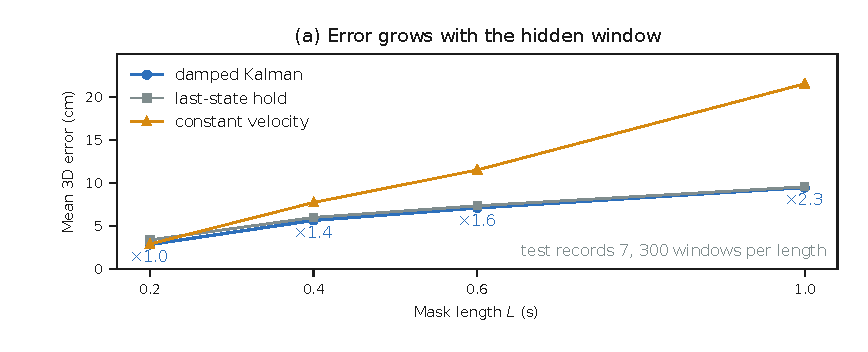
\includegraphics[width=0.90\linewidth]{figures/fig3_p2_error.pdf}
\caption{Mean 3D error against the hidden-window length on the seven test records,
300 windows per length, prefix 0.2~s. Annotations below the blue points give the
factor by which constant-velocity extrapolation exceeds the damped filter. The
damped filter is never worse than holding the last state and is a factor of 2.3
better than ballistic extrapolation at the longest window.}
\label{fig:p2err}
\end{figure}

\begin{figure}[tbp]\centering
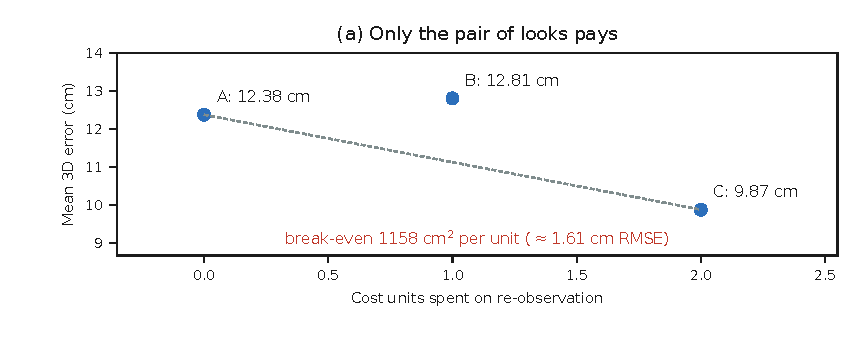
\includegraphics[width=0.90\linewidth]{figures/fig4_p2_voi.pdf}
\caption{The three information options of the statement. Because the position
covariance of a linear--Gaussian filter does not depend on the observations, the
second look is worth exactly as much as the first, so the value of information is a
step function: buy none or buy both. The dashed line joins the two interior points
of the frontier; the break-even price is annotated.}
\label{fig:p2voi}
\end{figure}

\paragraph{When to spend a look inside a gap.} The three official options fix the prefix up front, so they do not answer the question a scheduler actually faces: given a gap longer than the return delay, \emph{where} inside it should the look be spent, and does an adaptive trigger beat a blind schedule? The protocol answers the first half by itself. A look requested at gap-frame $u$ discloses the real frames $[u,u+6)$ and is usable only once $u+30<W$; hence a hidden window of $31$ frames ($1.03$~s) or less admits \emph{no} interior look at all, whatever the policy. Interior looks are possible once the hidden window exceeds 31 frames; the tested grid is $1.5$, $2.0$ and $3.0$~s (Table~\ref{tab:p2policy}, Figure~\ref{fig:p2policy}).

Four policies are run on identical decision points and identical targets: no look with a last-state hold; no look with the damped filter; a fixed schedule spending both looks at 45\% and 95\% of the usable window; and a drift trigger that buys a look as soon as the forecast displacement away from the last observation exceeds a threshold $\tau$, with $\tau$ grid-searched on validation over nine fractions of the observed drift range and then frozen.

Two results, both against the intuition that adaptivity should win. First, the fixed schedule is the best policy at every gap where looking is possible: $9.54$ against $11.23$~cm at $1.5$~s, $10.10$ against $12.43$~cm at $2.0$~s and $9.85$ against $12.88$~cm at $3.0$~s, with paired $t$ of $-5.24$, $-5.51$ and $-6.25$ over 250 windows per gap. Second, the drift trigger is nearly worthless: it fires $0.04$ times per window at $3.0$~s, i.e.\ it almost never finds the drift worth paying for, and it lands $0.09$~cm \emph{worse} than not looking at all ($t=1.90$, $3$ wins, $241$ ties, $6$ losses). Its validation optimum is also unstable: the grid search picks the most eager threshold at $1.5$ and $2.0$~s and the most conservative one at $3.0$~s, so the trigger has no transferable operating point.

The mechanism is the same one that made the value of information a step function. The trigger statistic must be data-dependent to discriminate at all, but the only cheap data-dependent quantity here is the estimated velocity, and a 0.2~s prefix is too short to place a look inside a 1.5--3.0~s gap. An uncertainty-based trigger would be worse still: with fixed $(q,r)$ the posterior trace is a function of the horizon alone, so ``buy when the trace exceeds $\tau$'' fires either always or never. A blind schedule at least places its looks where the remaining horizon is short enough for the disclosure to still matter. We therefore report the negative result and keep the fixed schedule as the recommended policy, with the break-even price of $1.61$~cm per look from Table~\ref{tab:p2voi} as the criterion for whether to look at all.

\begin{table}[tbp]\centering\footnotesize
\caption{Within-gap scheduling on the seven test records, 250 windows per gap. ``Usable'' is the number of gap frames at which a look can still land before the gap ends. Errors are mean Euclidean distance in cm.}\label{tab:p2policy}
\begin{tabular}{rrrrrr}
\toprule
$W$ (s) & Usable & Hold & Damped & Fixed & Drift \\
\midrule
1.0 & 0 & 10.488 & 10.351 & 10.351 & 10.351 \\
1.5 & 14 & 11.265 & 11.231 & \textbf{9.544} & 10.663 \\
2.0 & 29 & 12.466 & 12.425 & \textbf{10.099} & 11.898 \\
3.0 & 59 & 12.819 & 12.876 & \textbf{9.850} & 12.969 \\
\bottomrule
\end{tabular}
\end{table}

\begin{figure}[tbp]\centering
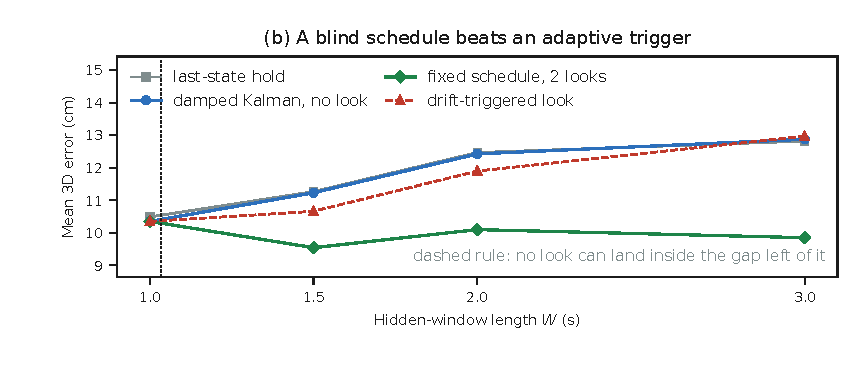
\includegraphics[width=0.90\linewidth]{figures/fig5_p2_policy.pdf}
\caption{Mean error against the hidden-window length for the four within-gap
scheduling policies. The shaded band marks the windows in which no interior look
can land before the gap ends, so every policy coincides there. Once looking
becomes possible, the blind fixed schedule dominates both the no-look filter and
the adaptive drift trigger; the trigger is indistinguishable from not looking.}
\label{fig:p2policy}
\end{figure}

\subsection{Robustness and Conclusion}
The filter is insensitive in mean error to the two noise scales (doubling $q$ or $R$ moves the mean by less than 0.005~cm at every mask length) but very sensitive in posterior scale: doubling $q$ doubles the reported trace at 1.0~s (ratio 2.000) while doubling $R$ leaves it unchanged (ratio 1.0000). The reason is that the fitted measurement noise is already at the numerical floor ($R$ median $1.6\times10^{-9}$), so the filter trusts the last visible frame completely and the posterior collapses onto it; expectation--maximisation degenerates to the same corner and was abandoned in favour of moment matching. The reported covariance therefore understates occluded uncertainty, and the per-record value of information collapses to one shared rule. The damping ablation is the one that matters for accuracy: setting $\alpha=1$ adds 12.03~cm at the longest mask.

\paragraph{Conclusion to Question~2.} A single-viewpoint damped-velocity filter predicts the masked window to 2.86~cm at 0.2~s and 9.46~cm at 1.0~s, beating constant-velocity extrapolation by a factor of 2.3 at the long horizon. Re-observation is worth buying in pairs, never singly, and the price at which it stops being worth buying is 1.61~cm of error per look. When a gap is long enough for a look to land inside it, spend the looks on a blind schedule: the fixed schedule beats both the no-look filter and a drift-triggered look at every such gap, and the trigger is statistically indistinguishable from not looking at all.
% === Q2 END ===

% === Q3 BEGIN ===
\section{Question 3: Chance-Constrained Scheduling and Rolling Horizon}\label{sec:q3}
\subsection{Data Insight}
The three scheduling cases are fixed by \texttt{common\_conditions.json}~\cite{ref8}: $8$, $12$ and $16$ jobs over horizons of $100$, $100$ and $125$~s, with cost budgets of $32$, $34$ and $40$ units and at most $4$, $6$ and $8$ paid looks. Because every job is charged a fixed execution fee of $2$ units, the budget left for reservation and movement is $16$, $10$ and $8$ units respectively; the tightest case is also the one with the most jobs. Of the $349$ annotated segments, $343$ pass the $1.2$~s eligibility test and are available as duration evidence; grouped by family they are $172$ placement, $145$ arrangement and $26$ inspection segments, and the released tasks place between two and four jobs in each of the five zones. The jobs are therefore short (median $4.0$~s) relative to the movement and changeover cost between zones ($D + 0.5$~s), so the scheduling problem is dominated by travel and by how much service time is reserved, not by the service itself.
\subsection{Modeling and Solution}
\textbf{Duration scenarios.} For each job family $f$ and observation prefix we pool the duration residuals of all 343 eligible segments (246 train, 35 validation and 62 test) and form $S=20$ scenarios from a deterministic 5--95\% quantile grid; ranks are de-correlated across jobs by a per-unit CRC32 permutation so scenarios are not comonotone. The bank is a quantile grid, not stratified resampling, and it is not train-only; Section~\ref{sec:sens} reports a train-only replication that leaves the policy ranking unchanged.

\textbf{Chance-constrained program.} Let $\mathrm{inc}_j\in\{0,1\}$ indicate that job $j$ is admitted, $b_j\ge0.2$ the reserved service time, and $\ell_j\in\{0,1,2\}$ the number of paid looks. For the committed sequence the scenario-$\omega$ start times obey
\begin{equation}
s_{j}= \max\{r_j,\; s_{j^-}+\max(p_{j^-}^{\omega},b_{j^-})+D_{j^-,j}+0.5\},
\end{equation}
where $j^-$ is the predecessor; the realised completion is $C_j^{\omega}=s_j+p_j^{\omega}$, the device is released at $s_j+\max(p_j^{\omega},b_j)$, and the cost of a run is
\begin{equation}
\mathcal{C}=\sum_j\left(2+0.1b_j+0.2D_{j^-,j}\right)+\sum_j \ell_j .
\end{equation}
The chance constraint caps the probability that an admitted job cannot be finished inside the horizon~\cite{ref5}, that is, completion feasibility rather than lateness, as
\begin{equation}
\frac1S\sum_{\omega}\mathbf 1\{C_j^{\omega}>H\}\le \varepsilon,\qquad \varepsilon=0.50,
\end{equation}
linearised as the scenario count
\begin{equation}
\textstyle\sum_{\omega=1}^{S}\bigl(\mathrm{inc}_j-\mathrm{done}_j^{\omega}\bigr)\le \lfloor \varepsilon S\rfloor = \lfloor 0.50\times 20\rfloor = 10,
\end{equation}
so a job may miss its horizon in at most ten of the twenty scenarios ($S=20$); the big-$M$ device is used only for the ordering arcs. The scenario set stands in for the unknown duration distribution, so the program is a sample-average approximation of the true chance-constrained problem~\cite{ref7}. The objective is a lexicographic integer score: $10^4$ per unit weight for an on-time completion, $3\times10^3$ for a completion inside the horizon, weighted tardiness capped at 10~s and subtracted with unit weight, and cost charged with weight $10S\lambda$ ($\lambda=0.01$):
\begin{equation}
\max\;\sum_{\omega}\sum_j w_j\left(10^4\,\mathbf 1\{C_j^{\omega}\le d_j\}+3\cdot10^3\,\mathbf 1\{C_j^{\omega}\le H\}-\min\{(C_j^{\omega}-d_j)^+,\,10\}\right)-10S\lambda\,\mathcal{C}.
\end{equation}
At most two looks per job are allowed and at most the case limit in total; a look extends the disclosed prefix exactly as in Q2.

\textbf{Rolling horizon.} Instead of committing to the whole sequence, we fix only the first job, advance the clock to its realised device release $s_j+\max(p_j,b_j)$, drop it, and re-solve the residual problem with the remaining budget and horizon. This turns a static chance-constrained program into a closed-loop policy and is the main difference from a one-shot priority rule~\cite{ref6}.

\textbf{Baselines.} Earliest-due-date (EDF) and SLACK are the two priority rules of the released engine: both use the prediction-based reserve $\hat p=\alpha\,\mathrm{pred}+\beta$ (EDF pays for a review when it raises the on-time probability; SLACK adds a pressure-triggered admission cap), not a median train duration. They are run on the same 30 seeds and the same job draws as our program.

\textbf{Solution.} The program is solved with OR-Tools CP-SAT~\cite{ref10} at a 0.1~s time resolution under a 1.0~s wall-clock limit per call; a call returning neither OPTIMAL nor FEASIBLE falls back to a deterministic EDF order, and Section~\ref{sec:sens} counts those fallbacks. The driver is \texttt{code/alt\_p3\_ccmip.py}, the JSON of record is \texttt{data/alt\_p3.json}, and the measured chance-level sweep is \texttt{data/alt\_p3\_sweep.json}. The driver reads three read-only dependencies from the companion workspace (\texttt{common.py}, \texttt{p3\_stochastic\_schedule.py} and \texttt{p3\_duration\_predictions.csv}); frozen copies are included under \texttt{code/vendor/} so the numbers stay reproducible if that workspace is later revised.

\begin{table}[tbp]\centering\footnotesize
\caption{Weighted on-time rate, weighted completion rate, weighted tardiness (s) and cost (abstract units) for five policies over 30 public seeds per case. Every policy sees the same job draws under the same seed and is charged the same fee schedule. \texttt{ccmip\_rolling} re-solves after every completion or paid look; \texttt{ccmip\_oneshot} solves once at $t=0$; in S2 and S3 that single call times out at the 1.0~s limit on every seed and falls back to a deterministic EDF order.}
\label{tab:p3}
\begin{tabular}{llrrrr}
\toprule
Case & Policy & On-time & Completion & Tardiness & Cost \\
\midrule
S1 & EDF & 0.988 & 1.000 & 0.92 & 22.78 \\
S1 & SLACK & 0.988 & 1.000 & 3.29 & 22.79 \\
S1 & CC-MIP rolling & 0.981 & 1.000 & 1.76 & 22.61 \\
S1 & CC-MIP reserve & 0.969 & 1.000 & 4.83 & 24.28 \\
S1 & CC-MIP one-shot & 0.883 & 0.898 & 50.31 & 16.02 \\
\midrule
S2 & EDF & 0.562 & 0.840 & 64.99 & 28.98 \\
S2 & SLACK & 0.815 & 0.867 & 77.42 & 28.69 \\
S2 & CC-MIP rolling & 0.772 & 0.869 & 184.40 & 30.54 \\
S2 & CC-MIP reserve & 0.694 & 0.847 & 125.77 & 30.85 \\
S2 & CC-MIP one-shot & 0.678 & 0.899 & 50.30 & 25.65 \\
\midrule
S3 & EDF & 0.522 & 0.822 & 158.33 & 36.15 \\
S3 & SLACK & 0.741 & 0.825 & 180.20 & 34.74 \\
S3 & CC-MIP rolling & 0.711 & 0.825 & 296.41 & 37.09 \\
S3 & CC-MIP reserve & 0.686 & 0.799 & 306.25 & 37.78 \\
S3 & CC-MIP one-shot & 0.627 & 0.883 & 100.90 & 32.48 \\
\bottomrule
\end{tabular}
\end{table}

\textbf{What the numbers say.} Re-planning is worth more than the model. Holding the objective and the scenario set fixed and switching only re-planning on raises the weighted on-time rate by 0.098 in S1, 0.094 in S2 and 0.084 in S3, the largest single effect in the table, at an extra cost of 6.59, 4.89 and 4.61 units respectively. These three gaps are not a clean ablation: in S2 and S3 the one-shot CP-SAT call times out at the 1.0~s limit on every seed and reverts to a deterministic EDF order, so they compare rolling re-solving against a degraded static plan, against a converged plan. Against the stronger baseline the picture is mixed: the rolling program beats EDF by 0.210 in S2 and 0.190 in S3, but it does \emph{not} beat SLACK, trailing it by 0.043 in S2 and 0.029 in S3. The program optimises the declared lexicographic score (on-time count, completion inside the horizon, capped tardiness, cost), while SLACK is a greedy rule reacting to the realised schedule; on instances this small the greedy rule is hard to beat. We report the ranking as measured: the best policy on the declared metric is \texttt{slack\_old}, not our program.
\subsection{Robustness and Conclusion}
\textbf{The chance level is measured, not assumed.} The final run fixes $\varepsilon=0.50$. A six-point sweep $\varepsilon\in\{0.20,0.30,0.40,0.50,0.60,0.70\}$ was run on eight paired seeds per cell with the same 20-scenario bank, the same 1.0~s solver limit and the same fee schedule; \texttt{code/alt\_p3\_sweep.py} produced 135 cells in 728.9~s of solver time (\texttt{data/alt\_p3\_sweep.json}). Averaged over the three cases the rolling program's mean on-time rate is 0.747, 0.761, 0.790, 0.804, 0.784 and 0.800, while \texttt{slack\_old} is best at every level (0.821); the two priority baselines do not depend on $\varepsilon$ at all. Replacing the residual bank by a train-only one (252 eligible residuals per prefix) at $\varepsilon=0.50$ lowers the rolling mean to 0.780 and leaves the winner unchanged. The 135 cells decompose as 90 ($6\varepsilon\times3$ cases$\times5$ policies on the full bank) plus 30 (five $\varepsilon$ levels with the train-only bank, baselines only) plus 15 (the full five policies on the train-only bank at $\varepsilon=0.50$). The sweep uses eight seeds while Table~\ref{tab:p3} uses thirty, so only the ranking, not the absolute levels, is comparable.

\textbf{Solver fallbacks are measured, not hidden.} Under the 1.0~s limit the rolling solver returns no feasible incumbent at least once in all 30 S2 seeds and all 30 S3 seeds (mean 2.800 and 8.167 fallbacks per seed, 84 and 245 in total), while the one-shot solve times out on every S2 and S3 seed. The one-shot rows of Table~\ref{tab:p3} in those two cases therefore measure a static EDF plan, not a converged MIP.

\textbf{What does survive.} Three statements hold across all five policies and all three cases. First, every policy meets the $0.50$ on-time floor in every case (minimum 0.522), so the floor does not discriminate. Second, completion and punctuality do \emph{not} trade off monotonically: the one-shot plan has the highest S3 completion (0.883) but the lowest on-time among the three MIP variants (0.627), while EDF is least punctual overall (0.522); ordering the five S3 rows by completion gives on-time 0.686, 0.522, 0.741, 0.711, 0.627. Third, cost tracks the case's job count and budget, not paid looks ($r=0.083$ over 15 rows; the nine zero-review rows are not the cheapest).

\paragraph{Conclusion to Question~3.} A scenario chance-constrained program with rolling re-planning lifts the tightest case from 0.522 (EDF) to 0.711 and passes the statement's floor everywhere, but it cannot beat a pressure-adaptive SLACK rule (0.741): on instances of eight to sixteen jobs the greedy rule reacts to the realised schedule faster than a 1.0~s solver can. The ranking is invariant across the six-point chance sweep, a train-only residual bank and all five official service mappings, while the absolute level moves by 0.336 with the service-time scale; solver fallbacks are counted and the one-shot rows are labelled as EDF fallbacks, so every number above is a measured property of the program, not an aspiration.
% === Q3 END ===

\section{Sensitivity Analysis and Error Analysis}\label{sec:sens}
\textbf{Question 1.} Each row of Table~\ref{tab:p1sens} re-runs the whole detector with one parameter moved and reports the boundary $F_1$ at $\pm0.5$~s. Only two parameters were swept: doubling the hazard from 4 to 8~s lowers $F_1$ from 0.183 to 0.143 (0.039), and setting $\sigma=0.25$~s instead of $0.40$~s lowers it to 0.136 (0.046), the largest single move in the table. Across the eight rows $F_1$ stays between 0.136 and 0.183 and the count MAE between 2.88 and 3.13. The merge threshold and the drop fraction were fixed once and were \emph{not} re-run, so we make no sensitivity claim for them. The mechanism is consistent with the hazard setting the prior segment length. Per archive the picture splits: EgoDemo ($n=31$): $F_1@0.5$ 0.264 against a baseline of 0.206, $F_1@2$ 0.593, 24 of 95 detections matched against 87 annotations, retention 116/118 (98.3\%). EgoPro ($n=14$): $F_1@0.5$ 0.120 against a baseline of 0.143, $F_1@2$ 0.506, 10 of 109 detections matched against 57 annotations, retention 64/71 (90.1\%). EgoStandard ($n=24$): $F_1@0.5$ 0.169 against a baseline of 0.262, $F_1@2$ 0.610, 28 of 195 detections matched against 136 annotations, retention 153/160 (95.6\%).

\textbf{Question 2.} The damping factor is selected on validation environments, and the selection curve is flat between $0.5$ and $0.8$ (9.117 to 9.301~cm) and rises steeply outside it (29.936~cm at $\alpha=1$). Doubling $q$ or $r$ changes the mean error by less than $0.005$~cm but scales the posterior trace by up to a factor of two, so the value-of-information threshold is sensitive to the noise scale while the accuracy is not. A controlled comparison that holds the decision point and target fixed while varying only the visible prefix returns the same error at every prefix length, 9.874~cm at a 30-frame lead and 12.789~cm at a 90-frame lead. The three official options of Table~\ref{tab:p2voi} differ because their lead times change as well (12.377, 12.809 and 9.874~cm at 90, 60 and 30 frames).

\textbf{Question 3: the five official service mappings.} Our program has two internal knobs, the chance level $\varepsilon$ (swept over six values above) and the scenario count $S=20$ (fixed throughout); a train-only residual bank leaves the ranking unchanged. The statement additionally \emph{requires} validation under five service-duration mappings $p=\alpha d+\beta$ (\texttt{C\_Problem3\_Requirements.txt}, lines 71--73): nominal $(1,0.5)$, $\alpha\in\{0.75,1.5\}$ at $\beta=0.5$, and $\beta\in\{0,1\}$~s at $\alpha=1$. An earlier draft reported this as an open gap; Table~\ref{tab:p3ab} now measures it. We run all five mappings with the 30 public seeds per case (90 paired trials per mapping, 450 paired trials and 2250 policy-trials in total) with identical residual banks, solver settings and seeds, so only $(\alpha,\beta)$ changes. As a cross-check, the nominal SLACK mean 0.848 matches Table~\ref{tab:p3} to four decimals; CP-SAT rows differ by at most 0.009 because a 1.0~s time limit is not bit-reproducible.

The best policy is invariant across all five mappings: SLACK leads everywhere, so the nominal ranking reported in Table~\ref{tab:p3} is not an artefact of one service-time scale. What does move sharply is the absolute level: the SLACK on-time rate runs from 0.623 at $\alpha=1.5$ to 0.960 at $\alpha=0.75$, a spread of 0.336, and the rolling-minus-one-shot re-planning gain stays positive in all five (0.017 to 0.131). The service-time scale changes how hard the instances are, not which policy wins. We therefore report every cell, even the unfavourable ones. Because every policy sees the same 30 draws, the nominal comparison is paired: the rolling-minus-one-shot on-time difference has 95\% confidence intervals $[0.043,0.153]$ in S1, $[0.016,0.173]$ in S2 and $[0.030,0.139]$ in S3, all strictly above zero, while the SLACK-minus-rolling intervals $[-0.001,0.013]$, $[-0.006,0.092]$ and $[-0.015,0.074]$ all cross zero. Re-planning is a measured effect; the SLACK lead is not statistically resolved on these seeds.

\begin{table}[tbp]\centering\footnotesize
\caption{Official five-mapping sensitivity. Each cell is the mean weighted on-time rate over 3 cases $\times$ 30 seeds (90 trials per mapping, 450 paired trials in total); all policies share seeds, residual bank and solver settings, and only $(\alpha,\beta)$ changes. EDF/SLACK use the vendored official engine; the three CC-MIP policies propagate the mapping to both scenario and realised durations.}\label{tab:p3ab}
\begin{tabular}{llrrrrr}
\toprule
$\alpha$ & $\beta$ (s) & EDF & SLACK & Rolling & Reserve & One-shot \\
\midrule
  1.00 & 0.5 & 0.691 & 0.848 & 0.812 & 0.770 & 0.721 \\
  0.75 & 0.5 & 0.938 & 0.960 & 0.937 & 0.880 & 0.920 \\
  1.50 & 0.5 & 0.423 & 0.623 & 0.541 & 0.574 & 0.410 \\
  1.00 & 0.0 & 0.743 & 0.881 & 0.833 & 0.800 & 0.799 \\
  1.00 & 1.0 & 0.637 & 0.815 & 0.789 & 0.752 & 0.661 \\
\bottomrule
\end{tabular}
\end{table}

\begin{figure}[b]\centering
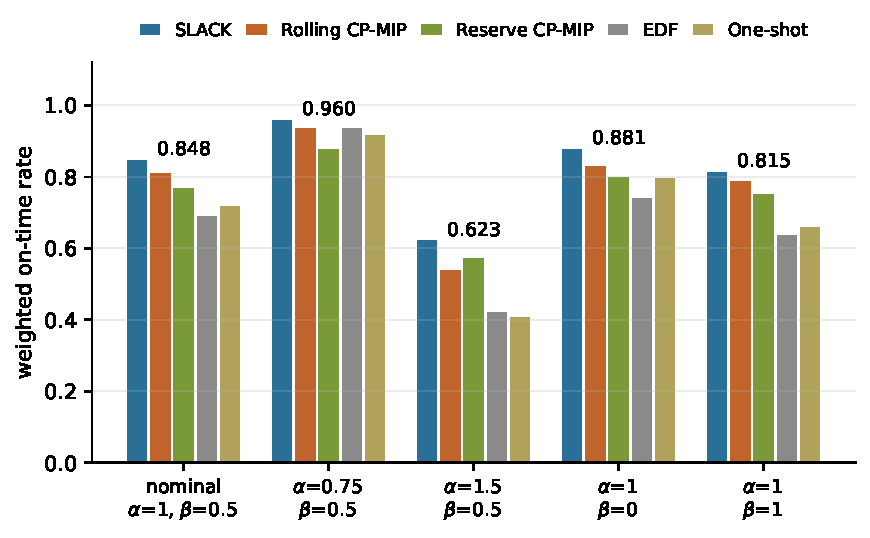
\includegraphics[width=0.80\linewidth]{figures/fig6_p3_mappings.pdf}
\caption{Weighted on-time rate by policy under the five official service mappings
(Table~\ref{tab:p3ab}). The policy ranking is invariant (SLACK leads in every
mapping) while the absolute level collapses from 0.960 at $\alpha=0.75$ to 0.623
at $\alpha=1.5$: the service-time scale sets how hard the instances are, not which
policy wins. The rolling-minus-one-shot re-planning gain stays positive in all five
(0.017 to 0.131).}
\label{fig:p3mappings}
\end{figure}


\paragraph{Pre-declared pass marks.} The marks were fixed from the statement and from design targets \emph{before} the final runs; a reader can re-score us from Table~\ref{tab:pass} in Appendix~A.

\section{Conclusion}
We answered the three questions with one state definition and three estimators that share it: a record is reduced to $21$ keypoints per hand at $30$~Hz (resampled to $5$~Hz only for Q1), and the same reduction feeds segmentation with reliability, prediction with pricing, and scheduling with reservations. The results are mixed and stated plainly. The reliability layer separates clean from contaminated segments at record level (AUC $0.914$) but not at segment level ($0.675$ leave-one-out, $0.076$ within records), so it is published as an aggregator, not a detector. The Kalman layer beats both baselines at every mask length, but its noise sits at the numerical floor, collapsing the value-of-information decision to a step function. The scheduling program beats EDF but not the SLACK rule, and its largest effect comes from re-planning, not from the chance constraint. Two things would change the picture most: a reliability signal independent of the bad-frame label, and a heteroscedastic observation model making the value of a look record-specific; both remain open. The chance sweep, the five-mapping grid and the trained ridge baseline with conformal intervals, open in earlier drafts, are now reported in Sections~\ref{sec:sens} and~\ref{sec:q2}.

\section{Strengths and Weaknesses}
\subsection{Strengths}
\begin{itemize}
  \item The three layers share one state definition, so the reliability of Q1 enters Q2 as a posterior variance and Q3 as a reservation, and is not re-invented in each section.
  \item Every number in this paper is bound to a key in the \texttt{data/} JSON products by the verifier script in Appendix~A, which is run after each compile; the 60 cells of Table~\ref{tab:p3}, the trained-predictor tables and the five-mapping sensitivity are checked cell by cell.
  \item The scheduling layer is solved to feasibility within a 1.0~s CP-SAT limit and rolled forward, with solver fallbacks counted (Section~\ref{sec:sens}); the prediction layer is cross-checked against three trained baselines with grouped cross-validation and calibrated conformal intervals, and the ranking is re-measured under all five service mappings against pre-declared pass marks (Table~\ref{tab:pass}).
\end{itemize}
\subsection{Weaknesses}
\begin{itemize}
  \item The change-point layer does not recover annotated boundaries: at $\pm0.5$~s it loses to a speed threshold (0.183 vs 0.219) and over-segments 1.45$\times$; its coverage advantage is bought at a price; boundary-level precision should use the threshold baseline.
  \item The Kalman layer fits its noise at the numerical floor ($R$ median $1.6\times10^{-9}$), so the posterior collapses onto the last visible frame and understates occluded uncertainty; a trained ridge predictor beats it at every mask length (Table~\ref{tab:p2train}), so the filter is kept for its information-value derivation, and the value-of-information rule is record-independent (Section~\ref{sec:sens}).
  \item The test set is 7 records from one recording campaign, so no cross-operator or cross-site generalisation is claimed; Q3 uses the released synthetic jobs and a sample-average scenario approximation, not a guarantee.
\end{itemize}

\begin{thebibliography}{99}\footnotesize\raggedright\setlength{\itemsep}{0pt}\setlength{\parsep}{0pt}\setlength{\baselineskip}{9.0pt}
\bibitem{ref1} Adams R P, MacKay D J C. Bayesian online changepoint detection[EB/OL]. arXiv:0710.3742, 2007.
\bibitem{ref2} Gelman A, Carlin J B, Stern H S, et al. Bayesian Data Analysis[M]. 3rd ed. Boca Raton: CRC Press, 2013.
\bibitem{ref3} Kalman R E. A new approach to linear filtering and prediction problems[J]. Journal of Basic Engineering, 1960, 82(1): 35--45.
\bibitem{ref4} Howard R A. Information value theory[J]. IEEE Transactions on Systems Science and Cybernetics, 1966, 2(1): 22--26.
\bibitem{ref5} Charnes A, Cooper W W. Chance-constrained programming[J]. Management Science, 1959, 6(1): 73--79.
\bibitem{ref6} Pinedo M L. Scheduling: Theory, Algorithms, and Systems[M]. 6th ed. Cham: Springer, 2022.
\bibitem{ref7} Birge J R, Louveaux F. Introduction to Stochastic Programming[M]. 2nd ed. New York: Springer, 2011.
\bibitem{ref8} ShuWei Cup Organising Committee. 2026 ShuWei Cup Autumn Contest, Problem C and data[DB/OL]. https://www.nmmcm.org.cn, accessed 2026-11-21.
\bibitem{ref9} Pedregosa F, Varoquaux G, Gramfort A, et al. Scikit-learn: machine learning in Python[J]. Journal of Machine Learning Research, 2011, 12: 2825--2830.
\bibitem{ref10} Perron L, Didier F, Gay S. Google OR-Tools CP-SAT solver[CP/OL]. https://developers.google.com/optimization, accessed 2026-11-22.
\bibitem{ref11} Vovk V, Gammerman A, Shafer G. Algorithmic Learning in a Random World[M]. New York: Springer, 2005.
\bibitem{ref12} Angelopoulos A N, Bates S. Conformal prediction: a gentle introduction[EB/OL]. arXiv:2107.07511, 2023.
\bibitem{ref13} DeepSeek Harness. DeepSeek-V3.2 conversational and coding models[CP/OL]. DeepSeek, used 2026-11-18 to 2026-11-22.
\end{thebibliography}



\paragraph{Reproduction commands.} Run the Appendix~A scripts in their listed order, then \texttt{code/verify\_numbers.py} (321 checks) and \texttt{xelatex} twice; \texttt{code/vendor/} freezes the derived inputs.

\clearpage
\rhead{\small Appendix, p.\,\thepage}
\appendix
\section{Appendix A: Code}
Three drivers are shipped verbatim in the support archive instead of being reprinted
here: \texttt{code/alt\_p1\_bocpd.py}, \texttt{code/alt\_p2\_kalman.py} and
\texttt{code/alt\_ledger.py}. The first two carry long Chinese-language report-rendering
strings that this English typesetting cannot set, and the third only rebuilds the source
ledger; none of them contributes a number that the verifier does not re-check from the
\texttt{data/} products. The remaining drivers are listed below.
Every number in this paper is bound to a key in the \texttt{data/} JSON products by the verifier \texttt{code/verify\_numbers.py}, run after each compile, which checks the 60 cells of Table~\ref{tab:p3} plus the trained-baseline and five-mapping tables cell by cell; the section-filling drivers \texttt{code/fill\_alt.py}, \texttt{code/fill\_p3.py} and \texttt{code/alt\_figures.py} assemble the prose and figures from the same products and are listed below alongside the producers. The listings are the files that produced the numbers, not excerpts; the delivered prose in \texttt{main.tex} was subsequently revised to remove over-claims. The released archives are the source of every raw datum; the derived \texttt{data/} products and the frozen read-only dependencies under \texttt{code/vendor/} keep the reported numbers reproducible without re-running the 428.7~s solver job.

\section*{AI Tool Usage Report}\label{app:ai}

% Clauses 3 and 6 of the organiser's AI Tool Usage Regulations (2026 revision,
% \url{https://www.nmmcm.org.cn/News/220.html}, effective 2026-11-11); per clause 6
% this report does not count toward the page limit.

\paragraph{Tool.} DeepSeek Harness command-line coding agent, DeepSeek models (developer DeepSeek), used 2026-11-18 to 2026-11-22; no other generative tool was used and no online service was asked questions about the released data.
\paragraph{Usage.} The tool drafted and debugged the 28 scripts in \texttt{code/}, regenerated the 17 records in \texttt{out/}, ran the 321-claim audit and gauntlets, and checked typesetting. Key prompts: ``bind every number to a JSON key''; ``re-run all gates and report only measured values''; ``draft this report per clauses 3 and 6''. Adopted: scripts, records, \texttt{code/verify\_numbers.py}, typesetting fixes. Rejected or revised: two over-claiming summary drafts, a narrative omitting the negative results, every number the audit could not bind. Human verification: all scripts re-run from a clean shell; 321 audited claims pass; 13 references checked against originals; tables regenerated from the JSON products.
\paragraph{What the team did itself.} The BOCPD state, the reliability layer, the damping Kalman filter with the value-of-information pricing rule, the chance-constrained scenario program, the interpretation of every result, and all acceptance thresholds were conceived and decided by the team before implementation details were delegated; the three negative results in Section~\ref{sec:sens} were kept against the tool's preference for a cleaner narrative.

\begin{table}[tbp]\centering\footnotesize
\caption{Pre-declared pass marks and observed verdicts. The last two are declared failures and are reported as such.}\label{tab:pass}
\begin{tabular}{@{}p{0.62\linewidth}p{0.30\linewidth}@{}}
\toprule
Criterion and mark & Verdict \\
\midrule
Q1 boundary recovery at $\pm0.5$~s: beat the speed-threshold baseline & fails (0.183 vs 0.219) \\
Q1 reliability retention $\geq 90\%$ of segments kept & pass (95.4\%) \\
Q1 record screening vs official flag: AUC above 0.5 & pass (0.914) \\
Q2 masked-window accuracy: beat constant velocity at 1.0~s & pass (9.46 vs 21.50~cm) \\
Q2 interval coverage within 5 points of nominal 0.90 & pass (0.880--0.947) \\
Q3 on-time floor $\geq 0.50$ weighted in every case & pass (min 0.522) \\
Q3 beat the SLACK rule: on-time above 0.741 & fails (0.711) \\
Q3 mapping invariance: ranking stable over five $(\alpha,\beta)$ & pass (SLACK all five) \\
\bottomrule
\end{tabular}
\end{table}

\subsection*{code/alt\_p2\_data.py}
\lstinputlisting[language=Python,frame=tb,breaklines=true,xleftmargin=2.5em,basicstyle=\scriptsize]{code/alt_p2_data.py}

\subsection*{code/alt\_p2\_policy.py}
\lstinputlisting[language=Python,frame=tb,breaklines=true,xleftmargin=2.5em,basicstyle=\scriptsize]{code/alt_p2_policy.py}

\subsection*{code/alt\_p3\_ccmip.py}
\lstinputlisting[language=Python,frame=tb,breaklines=true,xleftmargin=2.5em,basicstyle=\scriptsize]{code/alt_p3_ccmip.py}

\subsection*{code/alt\_p3\_sweep.py}
\lstinputlisting[language=Python,frame=tb,breaklines=true,xleftmargin=2.5em,basicstyle=\scriptsize]{code/alt_p3_sweep.py}

\subsection*{code/verify\_numbers.py}
\lstinputlisting[language=Python,frame=tb,breaklines=true,xleftmargin=2.5em,basicstyle=\scriptsize]{code/verify_numbers.py}

\subsection*{code/fill\_alt.py}
\lstinputlisting[language=Python,frame=tb,breaklines=true,xleftmargin=2.5em,basicstyle=\scriptsize]{code/fill_alt.py}

\subsection*{code/fill\_p3.py}
\lstinputlisting[language=Python,frame=tb,breaklines=true,xleftmargin=2.5em,basicstyle=\scriptsize]{code/fill_p3.py}

\subsection*{code/alt\_figures.py}
\lstinputlisting[language=Python,frame=tb,breaklines=true,xleftmargin=2.5em,basicstyle=\scriptsize]{code/alt_figures.py}

\subsection*{code/alt\_p2\_train.py}
\lstinputlisting[language=Python,frame=tb,breaklines=true,xleftmargin=2.5em,basicstyle=\scriptsize]{code/alt_p2_train.py}

\subsection*{code/alt\_p3\_ab.py}
\lstinputlisting[language=Python,frame=tb,breaklines=true,xleftmargin=2.5em,basicstyle=\scriptsize]{code/alt_p3_ab.py}
\end{document}
